\chapter{ATLAS探测器} \label{chap:ATLAS}
ATLAS探测器座落在LHC储存环的Point I,它有25米高,44米长,总重大约7000吨。ATLAS探测器内层是内部径迹探测器(ID),其被直径为2.3米的超导螺线管包围,该超导线圈提供平行于
束流方向,大小为2 T的磁场;紧挨着ID是量能器系统(EM),EM分为电磁量能器和强子量能器;最外层是$\mu$子探测器(MS)。本章将论述图~\ref{fig:ATLAS_schematic}所示的各个部分。

\begin{figure}[h]
\begin{center}
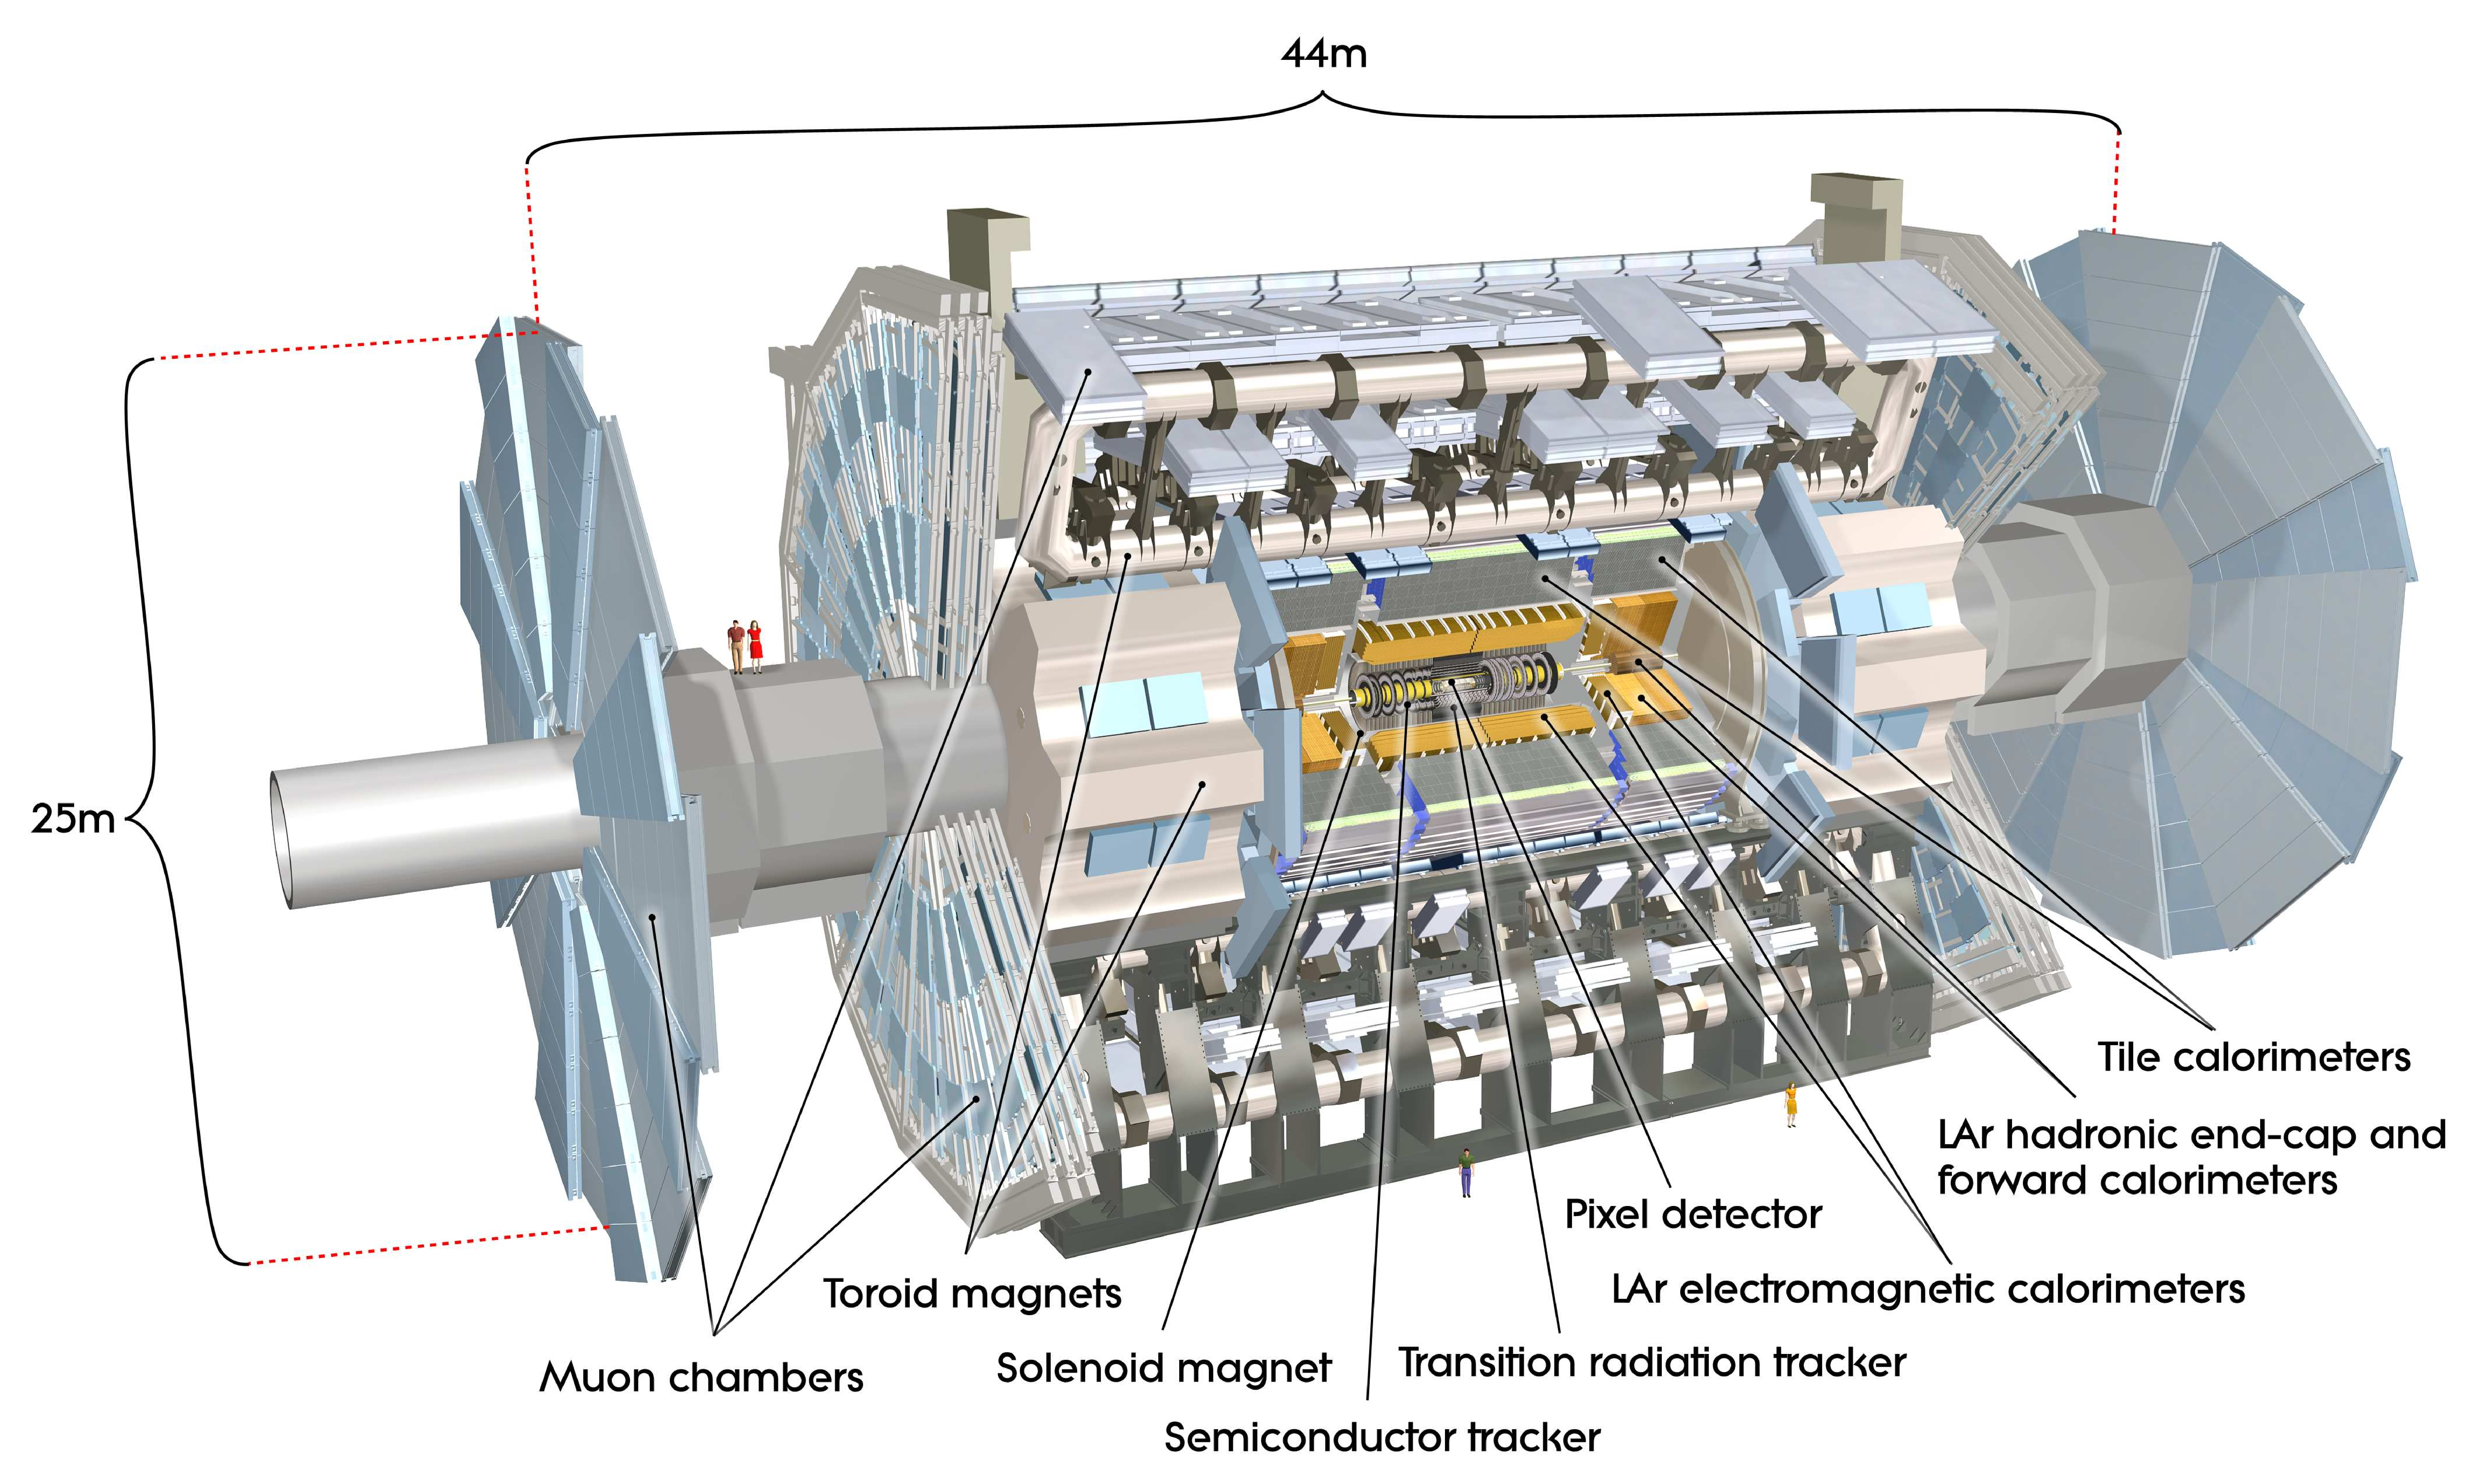
\includegraphics[width=0.9\textwidth]{fig/ATLAS_SE_Corrected7.pdf}
\caption{ATLAS探测器简图} \label{fig:ATLAS_schematic}
\end{center}
\end{figure}

\section{坐标系统}
ATLAS使用右手坐标系,其定义IP为原点,z轴为束流方向,正x轴指向环中心,正y轴则向上。在极角坐标系中,定义方位角$\phi$在(x, y)平面,大小从$-\pi$到$\pi$,极角$\theta$
从0到$\pi$,$\theta=0$时与正z轴同向。\\
赝快度定义为$\eta = -ln\tan(\theta/2)$($m\ll E$),更大的$|\eta|$意味着粒子更靠近束流方向,在ATLAS一般称为更前向。那么可以定义两个粒子的角距离$\Delta R=\sqrt{(\Delta\eta)^2+(\Delta\phi)^2}$。

\section{内部径迹探测器}
ATLAS内部径迹探测器主要用来精确寻迹(\pt > 0.1 GeV),可覆盖$|\eta|<2.5$。它包括三个子探测器,离束流中心距离从3.3 cm到101.6 cm,图~\ref{fig:ATLAS_ID_sideview}展示ID的
各个部分的分布。ID沉浸在通过铌钛超导螺线管产生的2 T轴向磁场中,线圈通过液氦冷却,温度为4.5 K。ID的强磁场可偏转带电粒子,通过测量径迹曲率可推出粒子动量。
\begin{figure}[h]
\begin{center}
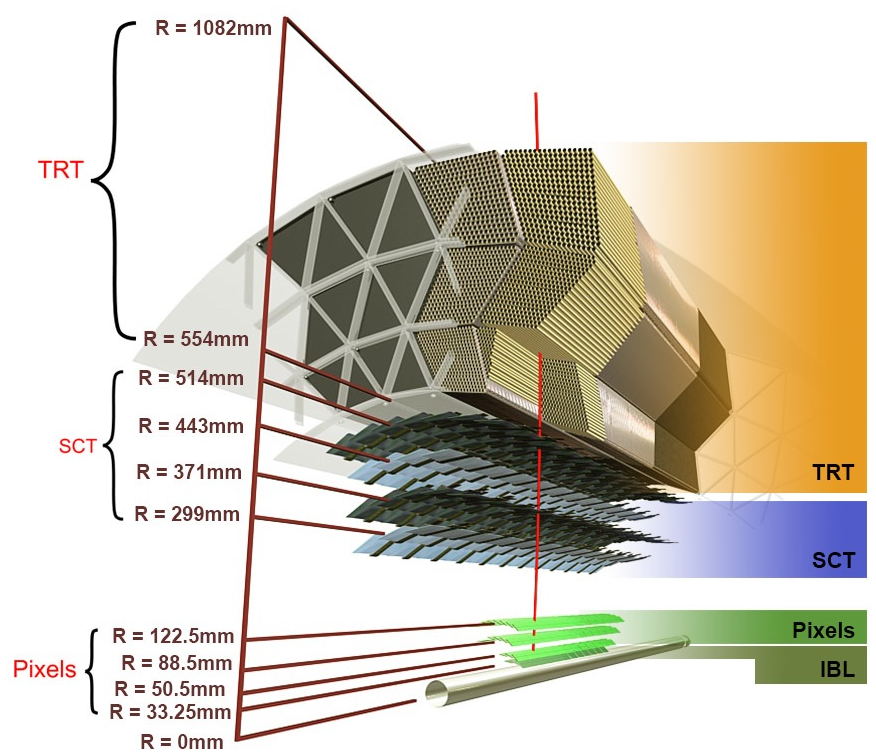
\includegraphics[width=0.9\textwidth]{fig/ATLAS_ID_sideview.png}
\caption{ATLAS内部径迹探测器} \label{fig:ATLAS_ID_sideview}
\end{center}
\end{figure}

%\subsection{像素探测器和IBL}
像素探测器(Pixel detector)围绕着束流中心,是离束流最近的系统,会经受最高密度的粒子束流,因此在ATLAS所有子探测器中具有最高的分辨率。Pixel在桶部区有四层,由1744个模块组成(module),端盖区有三层,含有288个模块。桶部区的最内层在Run 1和Run 2之间安装,主要用于提高\bjet 鉴别。每个Pixel模块含有46080个电子学读出道,Pixel探测器总共有8千万读出道。
模块面积为$50\times400 \mu m^{2}$,其位置分辨率可达10 $\mu m$(r-$\phi$),115 $\mu m$(z方向)。\\
硅微条探测器(Semiconductor silicon Strip Detector, 称SCT)桶部区有四层,端盖区有9层。SCT模块只能提供二维位置信息,所以每层SCT两个模块背靠背以一定角度粘贴在一起,当粒子穿过时,
就可提供三维位置信息。一般SCT的分辨率为17 $\mu m$(r-$\phi$),580 $\mu m$(z方向)。SCT的总读出电子学道为630万。\\
穿越辐射探测器(Transition Radiation Tracker,称TRT)由大约30万,直径为4 mm充满70\%氙气,20\% CF$_4$,10\%二氧化碳的漂移管组成,桶部区的漂移管与轴线平行,端部区的漂移管
则成辐射状,其总的电子学读出道为351,000。带电粒子穿过漂移管电离气体,电子在电压作用下达到管中心丝。桶部区(端部)只提供$r-\phi$(r-z)方向的位置测量。\\
TRT还有助于带电粒子识别。 TRT管与聚丙烯纤维和箔层交错:通过具有不同折射率的材料之间的边界区域的带电粒子发射X射线辐射,其强度与粒子本身的相对论γ因子成比例。 
通过这种X射线在吸管气体中的光电效应产生的电子产生的信号具有比源自经过的颗粒的信号更高的振幅。 
鉴于它们的轻质量,当它们的动量接近1 GeV时,电子开始产生过渡辐射,而π介子仅在O(100)GeV动量范围内开始辐射。 这条信息与电子识别算法有关。\\
ID可为粒子径迹重建提供36个着火点。联合这三个子探测器的信息,ID可测量\pt 低至400 MeV的粒子,其相应的动量可由如下公式~\cite{ATLAS_Collaboration_2008}描述:
\begin{equation}
 \frac{\sigma_{\pt}}{\pt}=0.05\%\pt\oplus1\%
\end{equation}

\section{量能器}
ATLAS量能系统~\cite{ATLAS_Collaboration_2008}包括几个具有不同技术和粒度的组件,涵盖非常大的范围(\abseta <4.9)。 所有组件都是采样量能计,带有被动非活性材料,可以产生电磁/强子簇射,这些簇射被连接到活性材料层,以检测一小部分进入的粒子能量。 能量通过测试束流~\cite{4436305,Davidek_2009}进行校准,并在碰撞数据中验证。 ATLAS量能器的布局如图~\ref{ig:Calorimeter_d3}所示。
\begin{figure}[h]
\begin{center}
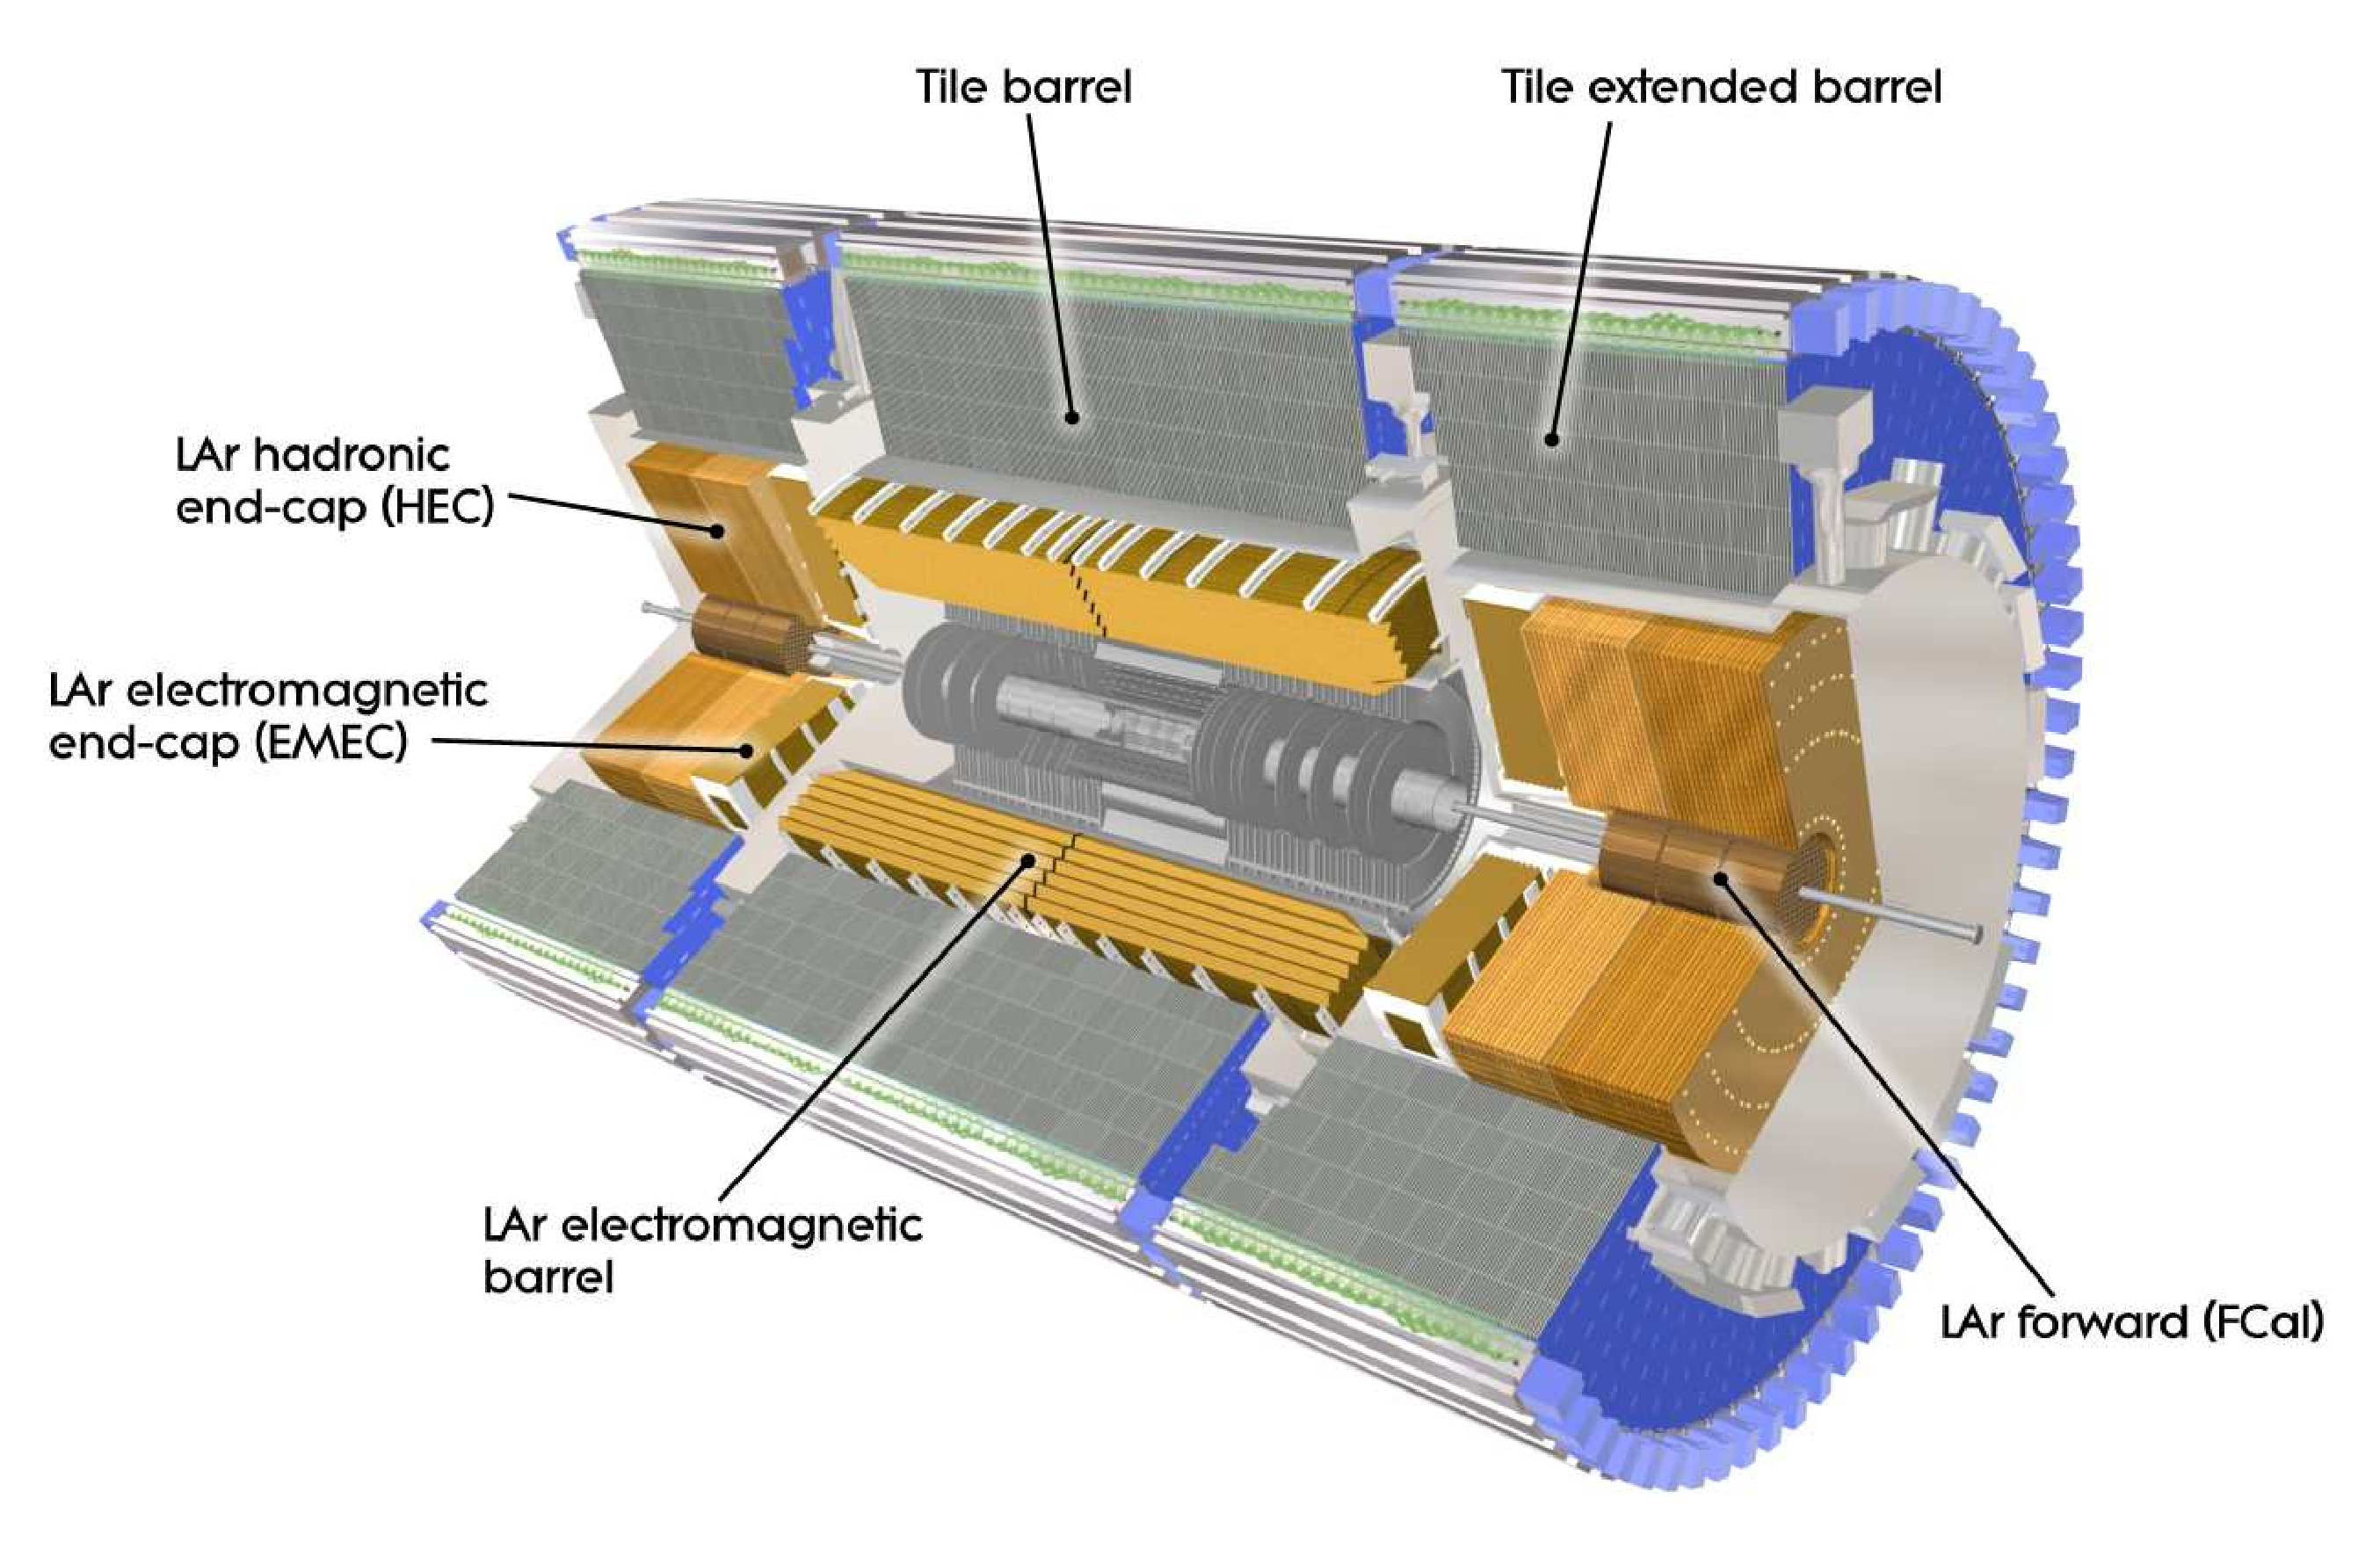
\includegraphics[width=0.9\textwidth]{fig/Calorimeter_d3.pdf}
\caption{ATLAS量能器布局} \label{fig:Calorimeter_d3}
\end{center}
\end{figure}
螺线管外部最里面的部分是电磁量能器(EM),专门用于电子和光子的能量测量。它使用液氩(LAr)作为活性介质,具有优异的辐射硬度和能量分辨率,并容易产生电磁簇射。
电极是镀有铜的电镀铜板,分成条带,构成读出单元。 EM桶部覆盖到\abseta = 1.4,端盖系统延伸到\abseta = 3.2。 它分为3-4层,具有类似手风琴的几何形状,可提供完整的$\phi$覆盖而不会出现死区,并且在ID探测范围内(\abseta <2.5)具有精细的$\Delta \eta\times\Delta\phi$分辨,最小值为0.025$\times$0.025,可以分辨$\pi0\rightarrow \gamma\gamma$。
EM厚度在桶部大于22个辐射长度(X0),在端盖区域中大于24倍X0,这样才能确保接收绝大多数电磁簇射。 过渡区域,即$1.37<\abseta<1.52$,由于大多数服务设施都位于此,能量测量部分缺乏,会有较差的能量测量表现。 EM能量分辨率可描述为~\cite{ATLAS_Collaboration_2008}:
\begin{equation}
\frac{\sigma_{E}}{E}=\frac{10\%}{\sqrt{E}}\oplus0.7\%
\end{equation}
强子量能器(HCal)包围着EM量能器,专门用于测量中子,$\pi$介子和中子等强子的能量。 桶区$\abseta<1.7$由三层钢-塑料闪烁体采样量能仪(TileCal)组成,其在$\eta = 0$时总厚度为9.7倍相互作用长度($\lambda$)。
这最大限度地强子簇射穿透HCal并到达外部$\mu$子光谱仪。 强子端盖量能器(HEC)覆盖$1.5<\abseta<3.2$,尽管使用铜作为被动材料并为平面状,但是与HCal采用相同的液态氩技术。 强子量能器的粒度比EM更粗,$\Delta \eta\times\Delta\phi$为$0.1\times0.1$,并且由于强子与材料核相互作用的性质,能量分辨率更差~\cite{ATLAS_Collaboration_2008}:
\begin{equation}
\frac{\sigma_{E}}{E}=\frac{50\%}{\sqrt{E}}\oplus3\%
\end{equation}
最后,3层前向热量计(FCal)覆盖$3.1<\abseta<4.9$以测量缺失的横向能量和前向喷注。 它利用LAr技术,分别用铜和钨作为第一层和最后两层的吸收材料。

\section{$\mu$子光谱仪}
$\mu$子光谱仪(MS)环绕着量能器,是ATLAS最外层的子探测系统,用于测量穿过ID和量能器的$\mu$子动量和位置。 MS系统有大约100万个电子学读出道,从半径5米延伸到10米,在\abseta =0处因为服务电缆有一个小间隙。
MS桶区由3个同心圆柱体组成,设计用于测量动量高于5 GeV的$\mu$子,其分辨率在100 GeV时为3\%。 端盖区有四个轮状部分,覆盖到$\abseta<2.7$。与ID类似,MS也可测量$\mu$子动量,
其磁场由大型空心环形磁体系统提供,大小在0.5~T和1~T之间。\\
$\mu$子室有两组系统:一组用于$\mu$子轨道的精确测量,第二组用于$\mu$子触发。精密腔室包括监测漂移管(MDT)\cite{Bauer:2016gyg}和阴极条带室(CSC)\cite{Argyropoulos:2009zz}。MDT涵盖$\abseta<2.7$的大部分区域,
 除了端盖最内层安装CSC区域$2.0<\abseta<2.7$。
 MDT由3cm直径的漂移管组成,其含有93\%氩和7\%CO$_{2}$的混合物。每根管具有单根钨-铼线,其在3kV的电压下操作,基于入射粒子产生的电离电荷的漂移时间可测量其相对位置。单管的典型空间分辨率低于100$\mu~m$,并且通过在每个腔室中使用3或4层管取决于其在检测器中的位置而改善至约50$\mu~m$。\\
 CSC由具有正交平面阴极的多丝比例室组成。它们可以处理更高的粒子流并且具有比MDT更高的辐射耐受性,因此被放置在粒子通量较大的前向区域$2<\abseta<2.7$。径向导线保持在1.9kV的电位,并与每个条状阴极保持2.5mm的距离。 在弯曲平面的CSC探测器寻迹分辨率约为60$\mu~m$并且具有高抗辐照性,因此用在MS的第一层。\\
 精密腔室通常具有长的电荷收集时间,MDT约为700ns,CSC约为40ns。收集时间的巨大差异是因为MDT和CSC的设计不同。MDT是在中心丝上施加电压的管,其中电场以$1/r^{2}$下降($r$是与中心丝的距离)。
而CSC是具有恒定电压差和恒定场的平坦腔室。两个专用触发室提供快速测量,用于触发决策。$\mu$子事件的触发系统基于电阻板腔(RPC)\cite{Aielli:2006hg}仪器在桶区域$\abseta<1.05$,而薄间隙腔(TGC)\cite{Majewski:1984ag}用于端盖区域。 
RPC由平行电极板组成,它们相距2mm并填充有$\text{C}_{2}\text{H}_{2}\text{F}_{4}$的气体混合物,工作在9.8kV的电压,有非常好的时间分辨率约为2ns。TGC由多线比例室组成,具有$\text{CO}_{2}$和$\text{n-C5H}_{12}$的气体混合物。TGC的阳极线距离带状阴极1.4mm,之间的电位差为2.9kV,时间分辨率为4ns。\\
环形磁铁在方位角平面上产生0.5T至1T的磁场。桶部中有八个矩形线圈,覆盖$\abseta <1.6$,每个端盖中有8个线圈,覆盖$1.4<\abseta<2.7$。线圈由铝,铜,铌和钛的混合物构成,并用液氦冷却至4.5K。MS的$\mu$子\pt~分辨率受到磁场不均匀性的限制。
\begin{figure}[h]
\begin{center}
 \begin{subfigure}[b]{0.45\textwidth}
      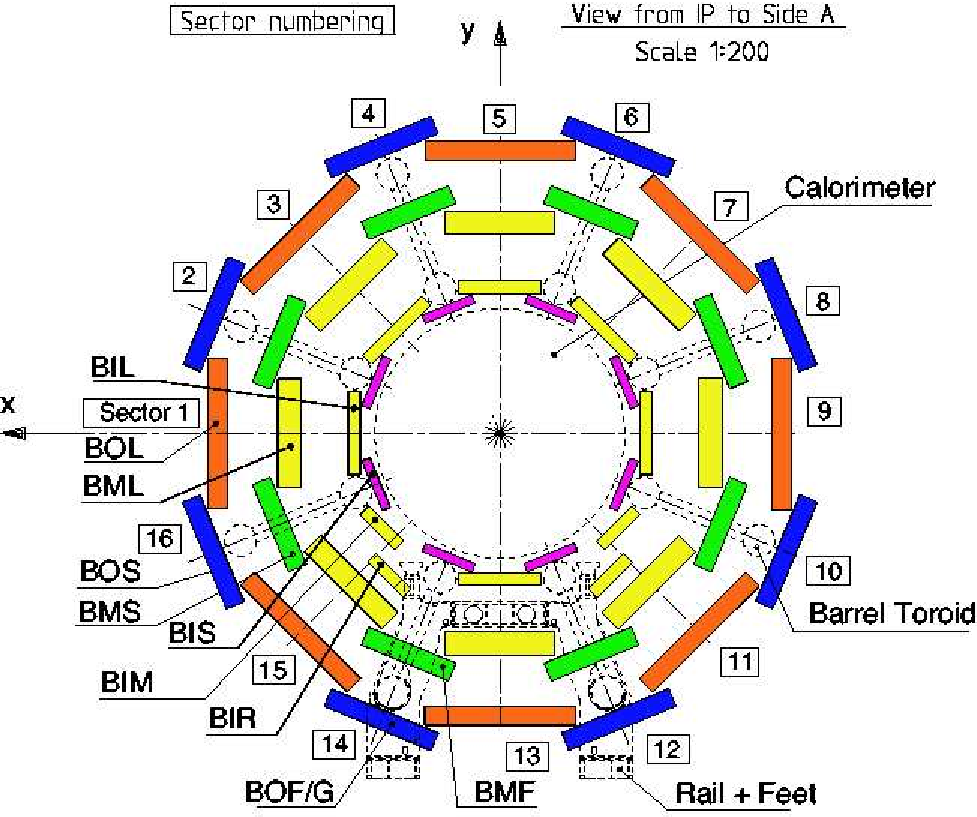
\includegraphics[width=\textwidth]{fig/Muon_sector_numbering.pdf}
      \caption{}
      \label{fig:muon_xy}
  \end{subfigure}
 \begin{subfigure}[b]{0.45\textwidth}
      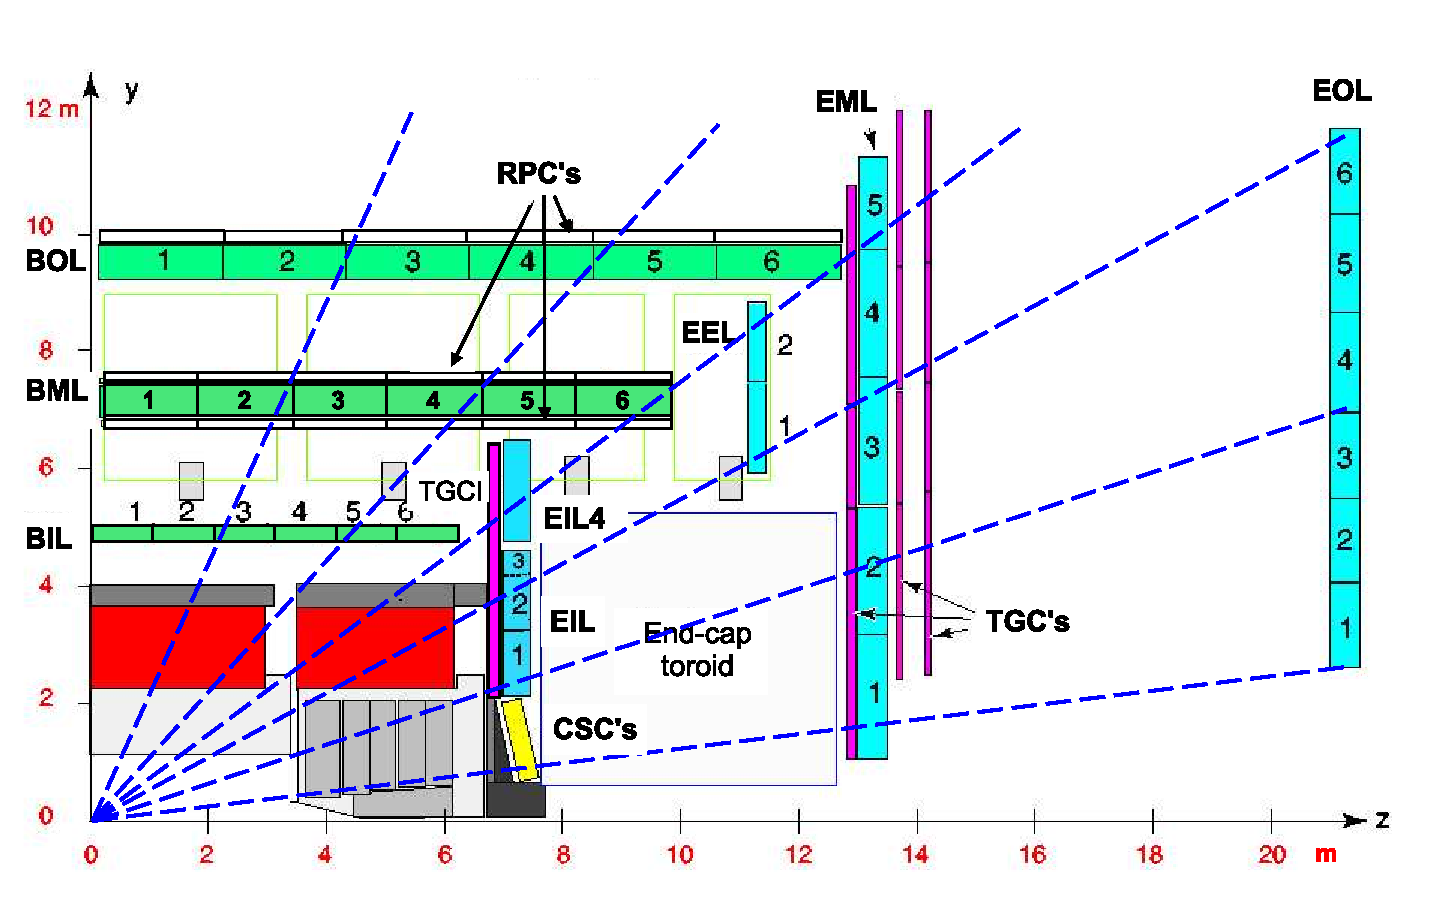
\includegraphics[width=\textwidth]{fig/Muon_rz_large_sect_6.pdf}
      \caption{}
      \label{fig:muon_rz}
  \end{subfigure}
\caption{(a) Cross-section of the barrel muon system perpendicular to the beam axis (non-bending plane), showing three concentric cylindrical layers of eight large and eight small chambers. The outer diameter is about 20m. (b) Cross-section of the muon system in a plane containing the beam axis (bending plane). Infinite-momentum muons would propagate along straight trajectories which are illustrated by the dashed lines and typically traverse three muon stations.} \label{fig:muon_overview}
\end{center}
\end{figure}

\section{触发和数据采集系统}
%由于数据存储容量和速率的限制,LHC每秒产生大量的事例必须经过实时筛选和在线触发\cite{Artz_2015},最终只有一小部分被记录。
%当前的ATLAS触发系统包括基于硬件使用来自量能器和$\mu$子系统粗略测量的触发(L1),以及基于软件的高级触发(HLT)。L1将事件发生率(这指bunch-crossing)从40 MHz降低到100 kHz,HLT进一步将其降低到1 kHz的平均记录速率\cite{Artz_2015}。ATLAS数据采集(TDAQ)系统的示意图如图\ref{fig:ATLAS_TDAQ}所示。
%L1触发系统执行初始事件选择并接受100 kHz速率的事件。它经过优化,可以快速做出决策。它联合量能器和MS的信息搜索高能量轻子,光子和喷注。电子和光子触发基于EM量能器中的能量沉积,这
%受限于EM本身分段。
%在强子量能器中,使用滑动窗口算法得到的触发元素形成的簇射最终构建候选喷注。
%一个触发元素是$0.2\times0.2(\eta-\phi)$单元格的总能量沉积,滑动窗口算法会在$4\times4$区域在特定阈值之上检查总$E_{T}$。$\mu$子触发基于触发室若干层着火点重合。
LHC束团间距为25ns,那么束团碰撞率为40MHz,质子非弹性散射率接近1GHz,平均pileup数为23.7,考虑到电子读出系统和数据存储能力的限制,ATLAS触发和数据采集系统(TDAQ)\cite{Aaboud2017}是探测器的基本组成部分,它负责决定是否为以后的离线研究保存事件。\\
TDAQ有两级:基于硬件的使事例率降低至100 kHz的Level-1触发器(L1),以及基于软件的高级触发器(HLT)系统。HLT使用40,000个CPU,并在一次LHC填充(fill)期间以1 kHz的平均速率选择事件,这是离线计算模型和存储可以处理的最大值。\\
L1触发器包括中央触发处理器(CTP),它处理来自L1量能器(L1Calo)和L1~$\mu$子(L1Muon)触发子系统的输入。L1Calo直接从量能器获取信息。L1Muon利用桶部($\abseta<1.0$)RPC和$1.0<\abseta<2.4$区的TGC进行测量。
为了应对更高的事件发生率并有效地选择感兴趣的物理事件,在2016年一个称为L1拓扑处理器(L1Topo)\cite{Simioni:2014nha}的新元素添加到L1中。L1Topo系统从L1Calo和L1Muon获取信息,可以计算不变质量等物理变量以用于L1决策。
由于L1电子设备的延迟为2.5μs,CTP也应用预防性死时间,设置L1连续两次接受决策之间的最短时间以避免重叠读出窗口,并限制在给定bunch-crossing数目内L1接受决策数以避免前端缓冲区溢出。\\
在L1触发接受之后,HLT使用更细粒度的量能器信息,来自MS的精确测量和来自ID的径迹信息来处理事件。为了最大限度地提高效率,HLT软件经过调整,使算法和选择尽可能接近离线重建。
HLT接受的事件最终存储在磁盘上,并导出到CERN计算中心进行离线重建。根据需要,HLT可以处理来自L1处识别的感兴趣区域(RoI)或来自完整探测器的信息。ATLAS触发系统的完整方案如图~\ref{fig:ATLAS_TDAQ}所示。
\begin{figure}[h]
\begin{center}
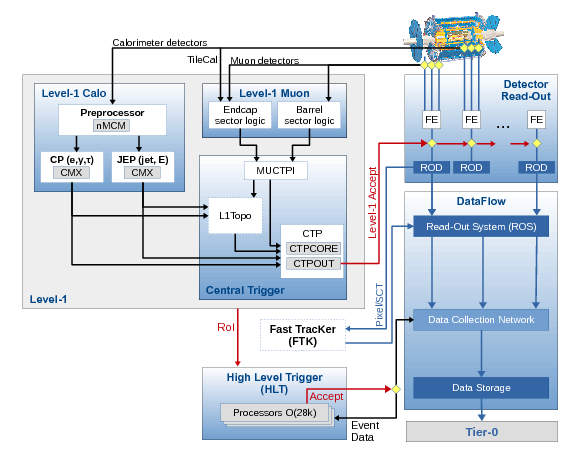
\includegraphics[width=0.75\textwidth]{fig/content_tdaq_figures_tdaq-run2-schematic.png}
\caption{The ATLAS TDAQ system in \RunTwo with emphasis on the components relevant for triggering. L1Topo and FTK were being commissioned during 2015 and not used for the results shown here.~\cite{Aaboud2017}} \label{fig:ATLAS_TDAQ}
\end{center}
\end{figure}
L1和HLT步骤的触发决策是对物理对象和筛选算法的一系列要求的结果,而这些定义了所谓的触发菜单。菜单中的主要触发器涵盖了各种ATLAS物理搜索所需的所有信号,包括电子,$\mu$子,光子,$\tau$轻子,喷注和丢失能量(MET)。
触发菜单组成和触发阈值针对若干亮度范围进行了优化,以便最大化实验的物理输出并且满足ATLAS探测器读出速率和带宽限制。许多ATLAS分析的主要特征信号,包括$hh\rightarrow 4W$搜索,是电子或者$\mu$子。 因此,在事件中需要存在至少一个$\pt>$25 GeV轻子的触发占据可用带宽的很大一部分,如图\ref{Trigger_singlelepton}所示。
\begin{figure}[h]
\begin{center}
\begin{subfigure}[b]{\textwidth}
\centering
      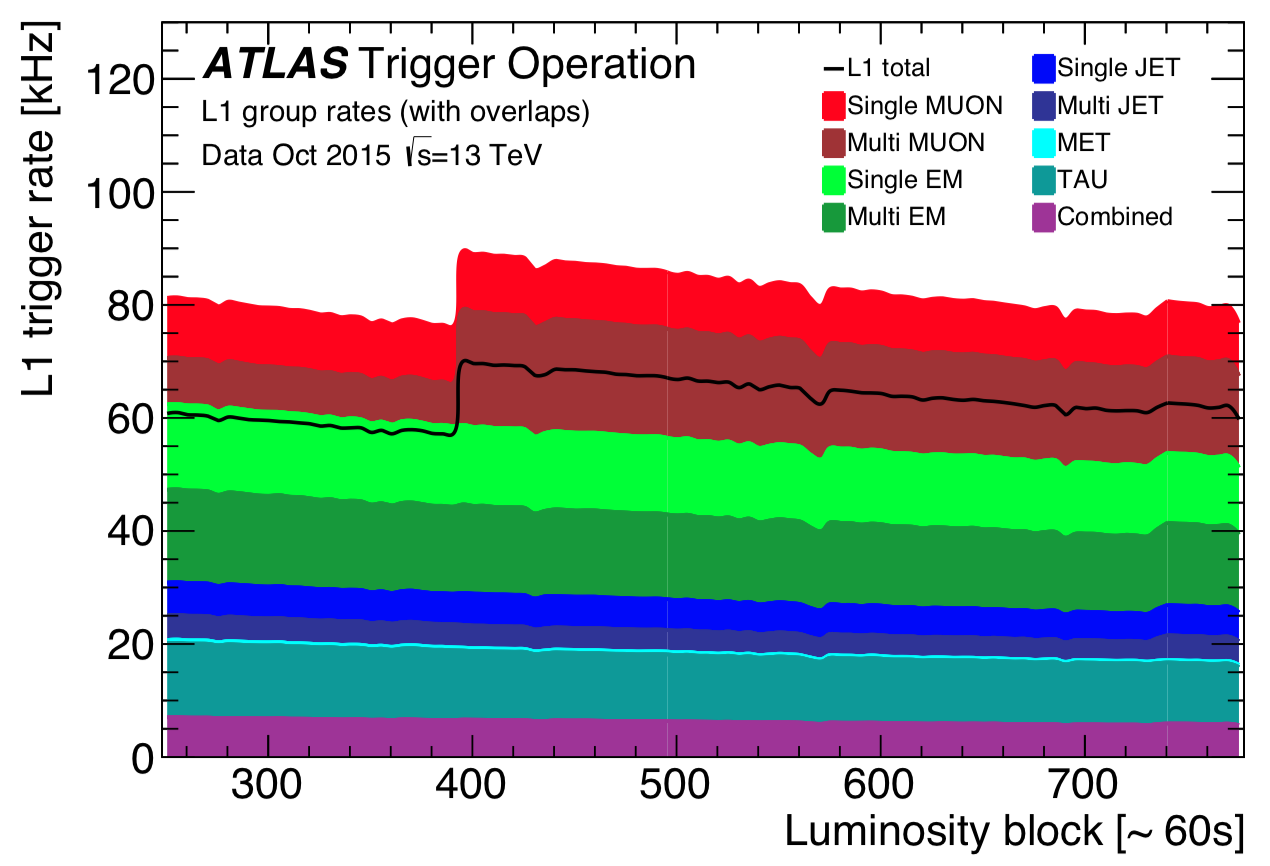
\includegraphics[width=\textwidth]{fig/content_menu_figures_Time_L1GroupRate_Stack.png}
     \caption{}
      \label{fig:L1_menu_rates}
  \end{subfigure}
 \begin{subfigure}[b]{\textwidth}
 \centering
      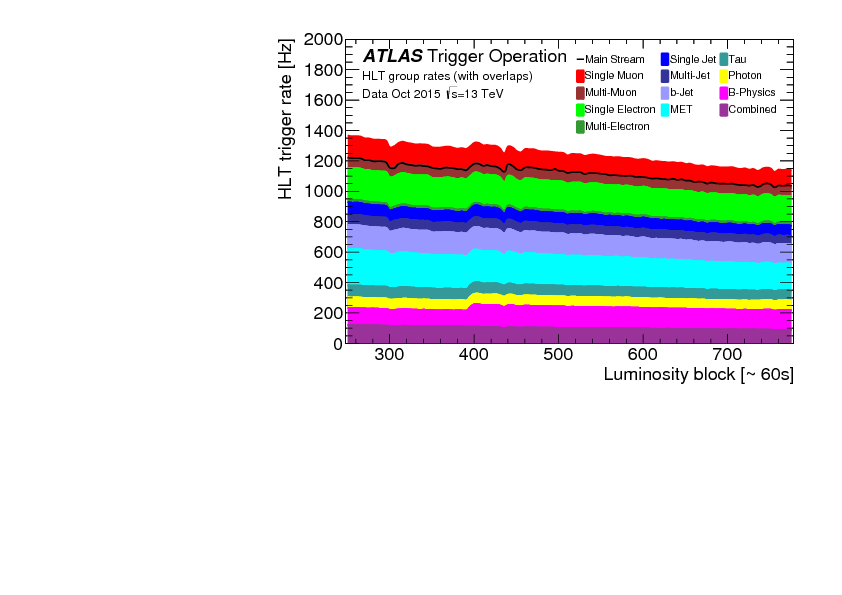
\includegraphics[width=\textwidth]{fig/content_menu_figures_Time_HLTGroupRate_Stack.png}
      \caption{}
      \label{fig:HLT_menu_rates}
  \end{subfigure}
\caption{(a) L1 and (b) HLT trigger rates grouped by trigger signature during an LHC fill in October 2015 with a peak luminosity of $4.5\times10^{33}\text{cm}^{-2}\text{s}^{-1}$. Due to overlaps the sum of the individual groups is higher than the (a) L1 total rate and (b) Main physics stream rate, which are shown as black lines. Multi-object triggers are included in the b-jets and tau groups. The rate increase around luminosity block 400 is due to the removal of prescaling of the B-physics triggers. The combined group includes multiple triggers combining different trigger signatures such as electrons with muons, taus, jets or MET.~\cite{Aaboud2017}} \label{fig:Trigger_singlelepton}
\end{center}
\end{figure}
